\chapter{Estudo de Caso} \label{cap:estudodecaso}

Foi realizado um estudo de caso para comparar o desenvolvimento de aplicações móveis utilizando ferramentas nativas e multiplataformas. Para isso, um aplicativo feito em \textit{iOS} 
nativo foi recriado utilizando o \textit{Ionic framework}. A seguir o aplicativo escolhido é detalhado em termos de funcionalidades e recursos utilizados. 

\section{Descrição do projeto selecionado} \label{sec:descricaodoprojeto}

Mini Farma é um aplicativo criado inicialmente para a plataforma \textit{iOS} que serve para controle dos medicamentos que as 
pessoas possuem em casa em suas ``farmacinhas'' particulares.

\begin{figure}[h]
  \centering
    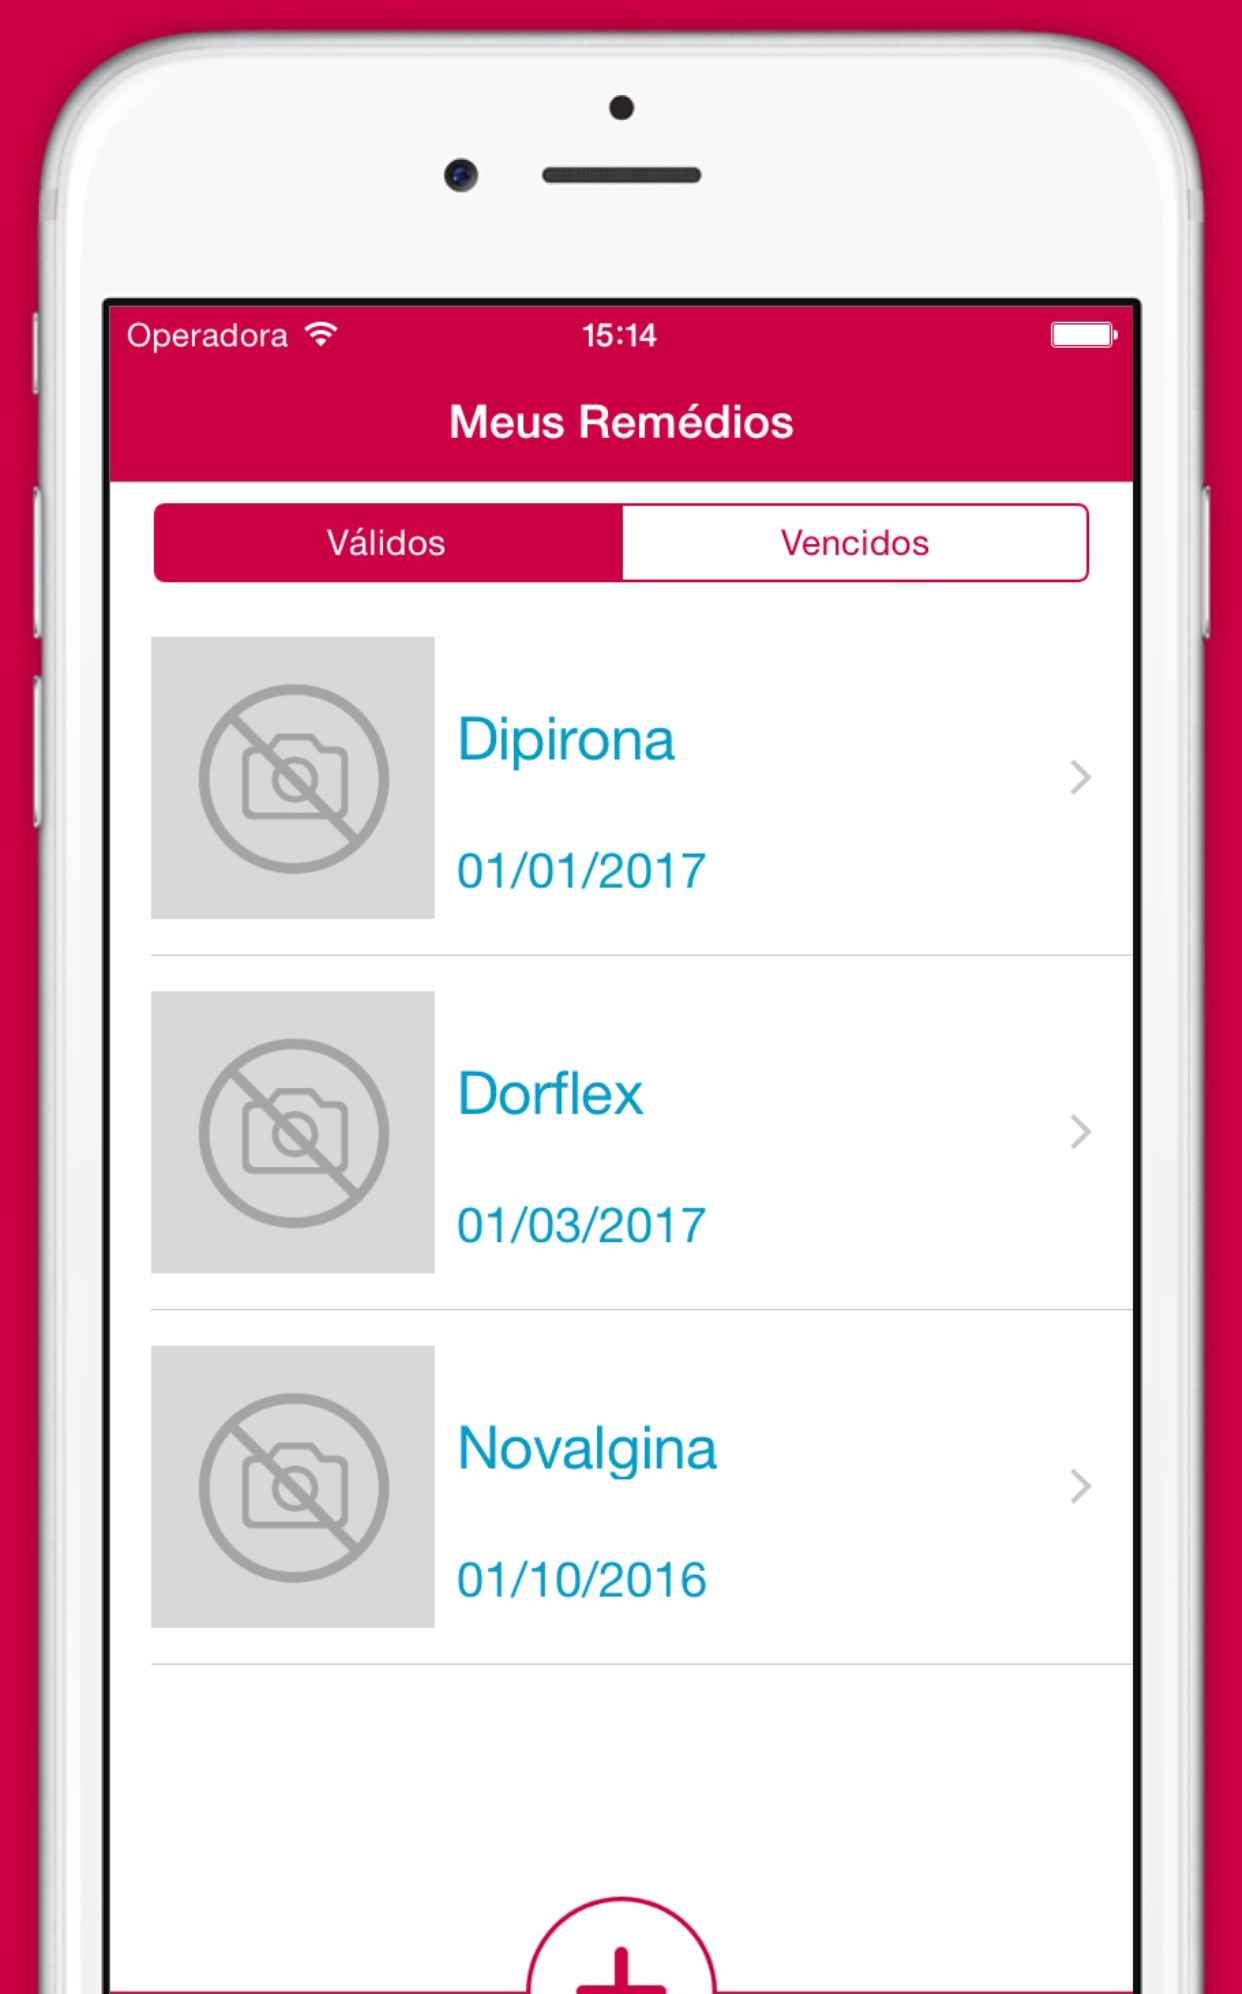
\includegraphics[width=0.5\textwidth]{minifarma}
    \caption[Tela inicial do aplicativo Mini Farma]{ Tela inicial do aplicativo Mini Farma. Fonte: Elaborado pelos autores.}
	\label{fig:minifarma}
\end{figure}

O aplicativo utiliza recursos nativos do sistema, os quais são descritos a seguir. 
\begin{itemize}
	\item \textbf{Localização geográfica}: Define a posição geográfica do dispositivo que o usuário está utilizando para salvar a 
    localização da farmácia onde ele comprou um medicamento para, caso seja necessário, explicar para alguém onde a 
    farmácia fica. Também é possível com base nessa localização da farmácia e do usuário, traçar uma rota para levá-lo diretamente à 
    farmácia em questão;
	\item \textbf{Notificações locais}: Diferente das notificações \textit{Push} as notificações locais são criadas e agendadas na central 
    de notificações do dispositivo e o sistema se encarrega de entregá-las corretamente de acordo com parâmentros definidos pelo aplicativo. 
    No caso do Mini Farma, as notificações são usadas para lembrar o usuário, na data e hora corretas, de que o mesmo deve tomar seus medicamentos;
	\item \textbf{Ligação}: As notificações podem conter ações que executam um determinado bloco de código dentro do aplicativo. No Mini Farma, 
    uma das notificações possíveis é a de aviso de pouca quantidade ou remédio esgotado, no caso do medicamento ter acabado. 
    Quando essa notificação é enviada, pode ser feita uma ligação diretamente pela ação da notificação para o número da 
    farmácia cadastrado no aplicativo. Dessa forma, o usuário pode solicitar uma nova quantidade de medicamento diretamente com a farmácia. 
	\item \textbf{Câmera}: Para facilitar a identificação dos medicamentos, é possível tirar uma foto com a câmera do dispositivo para 
    cada remédio cadastrado. Além de uma foto para o medicamento em si, é possível tirar uma foto da receita dele, caso haja;
    \item \textbf{Rolo de câmera}: Se o usuário já tiver uma foto que o ajude a identificar o seu medicamento ou da receita do mesmo salva 
    no rolo de câmera, é possível escolher a foto sem precisar tirar uma nova;
\end{itemize}

\textit{* Vale ressaltar, que com excessão da Ligação, todos os outros recursos nativos do sistema, precisam necessariamente serem autorizados pelo
usuário para funcionar. Caso o usuário não autorize, o aplicativo ficará com funcionalidades reduzidas.} 


Como banco de dados foi usado o SQLite, através do \textit{framework} externo e \textit{open-source FMDB}, 
disponível no \href{https://github.com/ccgus/fmdb}{Github};

A arquitetura do sistema foi criada com base no padrão de projeto MVC, possuindo Objetos de Acesso a Dados (DAO) para comunicação 
com o banco de dados. No entanto, o MVC tradicional difere em alguns aspectos do MVC usado no \textit{iOS}. 

No \textit{iOS} o MVC trás uma controladora ligada à classe de \textit{view}, que é chamado de \textit{ViewController}, que é responsável por 
criar a ponte entre a interação do usuário pela \textit{view} com as classes modelos. Dessa forma, as \textit{ViewControllers} têm a 
responsabilidade de repassar as entradas do usuário para a modelo e controlar a \textit{view} para apresentar os resultados que a modelo retornar.


Diferente do MVC tradicional, no qual a controladora apenas repassa as informações que estão entrando na fronteira da aplicação, 
as \textit{ViewControllers} têm, além dessa responsabilidade, também a responsabilidade de instanciar e gerenciar a \textit{view} no tocante
a organização dos elementos e apresentação das informações.


Outra observação sobre as diferenças entre os dois MVC's, é que no MVC tradicional pode haver uma controladora apenas 
para todas as modelos ou uma controladora por modelo, mas nenhuma ligada diretamente a uma \textit{view}, no entanto, no iOS há uma 
\textit{ViewController} por \textit{view}, podendo haver ainda uma controladora relacionada com cada modelo conforme o padrão tradicional do MVC.

%\textcolor{red}{\textit{TALVEZ SERIA BOM COLOCAR UMAS IMAGENS AQUI PARA MOSTRAR AS DIFERENCAS ENTRE OS DOIS MVCs GRAFICAMENTE, V-C-M E V-VC-C-M-DAO}}

\begin{figure}[h]
  \centering
    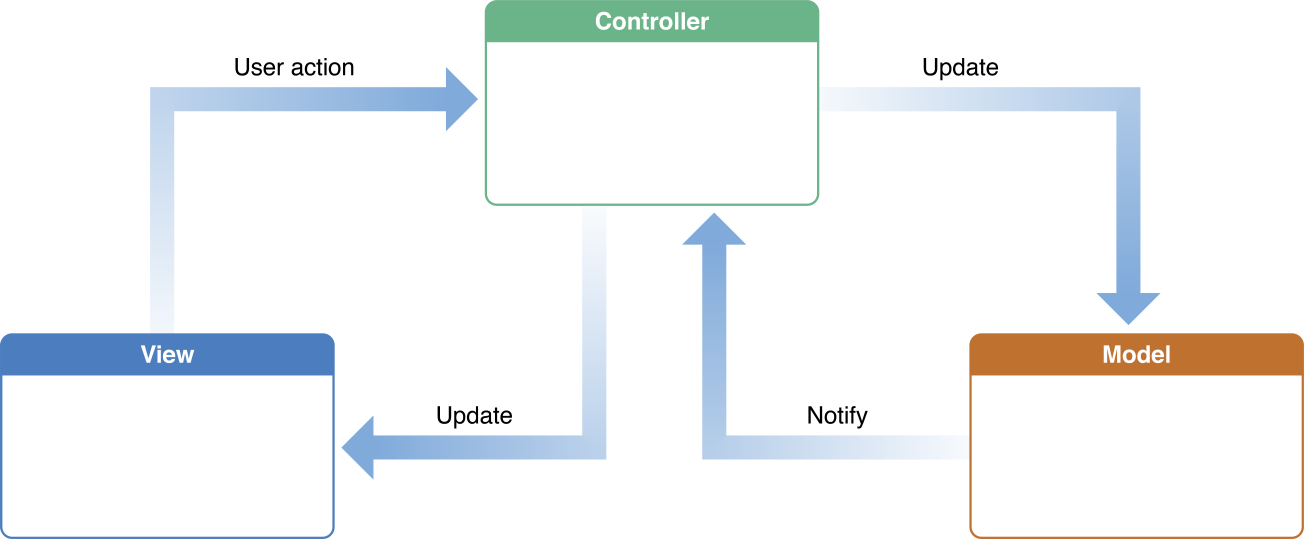
\includegraphics[width=1.0\textwidth]{mvc}
    \caption[Padrão \textit{Model-View-Controller}]{ Padrão \textit{Model-View-Controller}. Fonte: Apple Documentation.}
	\label{fig:mvc}
\end{figure}

\subsection{Ambiente de desenvolvimento} \label{subsec:ambientedesenvolvimento}
Nesta seção é apresentado todo o ambiente de desenvolvimento do \textit{app} Mini Farma quando foi feito originalmente para a plataforma \textit{iOS}. 
O projeto foi executado contando com uma equipe de dois integrantes com conhecimentos intermediários na plataforma \textit{iOS}. 
Os detalhes técnicos são listados a seguir.
\begin{itemize}
    \item \textbf{Máquinas}: Dois MacBook Pro Retina 13", processador \textit{Intel Core i5}, 8 GB de \textit{RAM};
    \item \textbf{Sistema Operacional das máquinas}: \textit{Mac OS X Yosemite} v10.10.5;
    \item \textbf{Sistema Operacional alvo do aplicativo}: iOS 8;
    \item \textbf{IDE}: \textit{Xcode} v6.4;
    \item \textbf{Linguagem de Programação}: \textit{Swift} v1.3;
    \item \textbf{Banco de dados}: SQLite v3.8.10.2;
    \item \textbf{Ambiente de suporte}: \textit{Plugin SQLite Manager} para \textit{Mozilla Firefox}, para criação do banco de dados;
    \item \textbf{Tempo de desenvolvimento}: Ambos os integrantes trabalharam no projeto quatro horas por dia de segunda à sexta por três semanas;
\end{itemize}

\section{Desenvolvimento multiplataformas do projeto} \label{sec:desenvolvimentomulti}

A partir do aplicativo feito em \textit{iOS}, foi construída uma versão utilizando o \textit{Ionic} para as plataformas \textit{Android} e \textit{iOS}.
Para a criação dessa versão do \textit{app}, a equipe foi alterada, mas permaneceu com dois integrantes, que são os autores deste trabalho.
No entanto, os integrantes não possuiam qualquer conhecimento prévio nos \textit{frameworks Ionic, AngularJS} e \textit{Cordova}
e apenas possuiam um conhecimento básico em \textit{HTML}, \textit{CSS} e \textit{JavaScript}. Os detalhes técnicos são listados a seguir.
   
\begin{itemize}
    \item \textbf{Máquinas}: Dois MacBook Pro Retina 13", processador \textit{Intel Core i5}, 8 GB de \textit{RAM};
    \item \textbf{Sistema Operacional das máquinas}: \textit{Mac OS X El Capitan} v10.11.5;
    \item \textbf{Sistema Operacional alvo do aplicativo}: \textit{iOS} 9 e \textit{Android} 4.4.2;%API 19
    \item \textbf{IDE}: \textit{WebStorm} v2016.1.1;
    \item \textbf{\textit{Frameworks}}:
    \begin{itemize}
        \item \textbf{\textit{Ionic}}: \textit{Copenhagen} v1.2.4*;
        \item \textbf{\textit{AngularJS}}: \textit{foam-acceleration} v1.4.3*;
        
        * Durante a execução deste trabalho, já haviam sido disponibilizadas as versões 2 do \textit{Ionic} e do \textit{AngularJS}, no entanto,
        os autores optaram por não utilizá-las por ainda se tratarem de versões \textit{beta} e portanto instáveis, o que poderia 
        impactar negativamente no desenvolvimento do projeto.
        
        \item \textbf{\textit{Cordova}}: v6.0.0;
    \end{itemize}
    \item \textbf{Linguagem de Programação}: \textit{JavaScript} v1.7. 
    \begin{itemize}
        \item \textit{HTML} 5 e \textit{CSS} 3 foram usados paralelamente para a criação da interface gráfica do aplicativo;
    \end{itemize}
    \item \textbf{Banco de dados}: SQLite v3.8.10.2;
    \item \textbf{Ambiente de suporte}: \textit{Google Chrome}, para \textit{debug} do aplicativo;
    \item \textbf{Tempo de desenvolvimento}: Ambos os integrantes trabalharam \textcolor{red}{XX} horas;
\end{itemize}

\subsection{Experiências de Desenvolvimento} \label{subsec:experienciasdev}

\textcolor{red}{PARECER SOBRE A UTILIZAÇÃO DO GOOGLE MAPS - A utilização do mapa se deu por meio da \textit{API Maps} do Google. Não houveram grandes dificuldades na criação do mapa e renderização do mesmo na tela. Apenas por meio de pesquisas e estudos na documentação
da \textit{API} já foram suficientes para a elaboração do que precisava ser feito. }

\textcolor{red}{nao é possivel debugar o ios pelo terminal, por causa da atualizacao do ios 9, por isso é necessario do xcode ou do safari, ou seja um mac}


\textcolor{red}{celulas colapsaveis na tela de add remedio}


\textcolor{red}{usar o banco na primeira controladora do sistema, cordova nao carrega antes da view}


\textcolor{red}{possibilidade de debugar com os navegadores, é possivel usar os navegadores para poder debugar enquanto esta rodando no simulador das plataformas}


\textcolor{red}{debug com alerta de javascript, nao eh falado em lugar nenhum, mas facilita muito. foi encontrado por pesquisas na comunidade on line}


\textcolor{red}{teve que criar tabs diferentes para ios e para android, pois a composicao original do aplicativo nao caia bem no android, entao foi necessario criar duas views para poder melhor adaptar ao android}


\textcolor{red}{ng-class nao funciona na ion-nav e foi muito dificil descobrir isso}


\textcolor{red}{passar dados de uma pagina para outra, semelhante ao protocolo do ios em questao de dificuldade}


\textcolor{red}{datepicker para selecionar data, foi utilizado um projeto disponivel no github para a exibição de um date picker para o cadastro de alertas, simples e fácil de se utilizar}


\textcolor{red}{problemas na hora de executar no iphone, o projeto não executa corretamente as vezes por motivo desconhecido}

